\chapter{Ausgewählte Aspekte}
\section{WCAG 2.1}
\label{wcag_2_1}
Die Web Content Accessibility Guidelines 2.1 (WCAG 2.1) sind im Dezember 2008 veröffentlicht worden und sind ein Standard, der weltweit verwendet wird, um Dienstleistungen im Web so barrierefrei wie möglich zu gestalten (vgl. W3C 2018, \cite{wcag_2_1_2018}, 18.08.2020). Somit können auch Menschen mit Behinderungen, wie etwa Sehschwäche, Blindheit, Hörverlust, Taubheit, körperliche oder kognitive Einschränkung, Sprachbehinderung, Lichtempfindlichkeit, Lernbehinderung oder Kombinationen dieser, das World Wide Web nutzen. Diese Richtlinien sind vom World Wide Web Consortium (W3C) am 5. Juni 2018 für Webanwendungen empfohlen worden.

Durch die Befolgung der Empfehlungen des W3C können Webdesigner und -entwickler, politische Entscheidungsträger, Käufer, Lehrer und Studenten beziehungsweise Schüler das WWW nahezu problemlos nutzen. Die WCAG 2.1 setzen sich aus allgemeinen Prinzipien, allgemeinen Richtlinien, prüfbaren Erfolgskriterien sowie einer Vielzahl an Techniken zusammen:

\begin{itemize}
	\item Es gibt vier \textbf{Prinzipien}, die die Grundlagen für die Web-Zugänglichkeit bilden: wahrnehmbar, bedienbar, verständlich und robust (englisch: perceivable, operable, understandable and robust).
	\item Die Prinzipien beinhalten insgesamt 13 \textbf{Richtlinien}, an die sich Entwickler halten sollen, um das Web zugänglicher zu machen. Sie sind zwar nicht prüfbar, helfen allerdings dabei die Erfolgskriterien besser zu verstehen und die Techniken besser umzusetzen.
	\item \textbf{Prüfbare Erfolgskriterien} werden dort eingesetzt, wo bestimmte Anforderungen und Tests für die Konformität erforderlich sind, wie etwa beim Entwurf, beim Kauf, bei Regelungen und bei vertraglichen Vereinbarungen. Es gibt drei Ebenen der Konformität, wobei die höchste AAA, die mittlere AA und die niedrigste A ist.
	\item \textbf{Ausreichende und beratende Techniken} dienen zur Erfüllung der Erfolgskriterien und als Beratung. Häufig vorkommende Misserfolge sind ebenfalls dokumentiert.
\end{itemize}

\mbox{}\\
Bei Erreichung der höchsten Ebene ist eine hundertprozentige Web-Zugänglichkeit jedoch nicht garantiert. Die WCAG 2.1 dienen ausschließlich als Anleitung, um das Web so barrierefrei wie möglich zu gestalten. Deshalb wird vom W3C empfohlen sich regelmäßig über den neuesten Stand zu informieren und sich mit anderen zu beraten. Folgende Bemerkung ist vom W3C veröffentlicht worden:\\

\mbox{}\\
''[...] Authors are encouraged to consider the full range of techniques [...] as well as to seek relevant advice about current best practice to ensure that Web content is accessible, as far as possible, to this community. [...]'' (vgl. W3C 2018, \cite{wcag_2_1_2018}, 18.08.2020)

\section{Web Components}
\label{web_comp}
Web Components sind eine Web-Technologie, die es den Entwicklern ermöglicht, selbstdefinierte HTML-Elemente zu erstellen und wiederzuverwenden (vgl. MDN Web Docs, \cite{moz_webcomp_2019}, 03.10.2020). Diese sind mit ihrem CSS und JavaScript gekapselt und sind somit vollständig von anderem Code getrennt. Mit einigen JavaScript Frameworks wie etwa Angular war es zwar bereits möglich wiederverwendbare HTML-Elemente zu definieren, allerdings nutzt jedes der Frameworks einen anderen Standard. Dies bedeutet, dass der Code in anderen Projekten in den meisten Fällen nicht verwendbar ist. Genau dieses Problem ist durch Web Components gelöst worden. Die Web Components bestehen aus drei Hauptbestandteilen:

\begin{itemize}
	\item \textbf{Customs Elements:} Ein Satz von JavaScript APIs zur Definition von benutzerdefinierten Elementen.
	\item \textbf{Shadow DOM:} Ein Satz von JavaScript APIs zum Hinzufügen eines DOM-Elementes mit gekapselten Shadow-DOM-Elementen, welches separat vom Hauptdokument DOM gerendert wird. Dadurch ist es möglich jegliche Funktionalitäten isoliert zu definieren, sodass der Programmierer keine Rücksicht auf Kollisionen mit anderen Dokumenten nehmen muss.
	\item \textbf{HTML Templates:} Markup-Vorlagen, die innerhalb der Elemente \texttt{<template>} und \texttt{<slot>} geschrieben werden, werden nicht auf der dargestellten Seite abgebildet. Diese sind dafür da, um sie mehrmals als Vorlage eines benutzerdefinierten Elements zu verwenden.
\end{itemize}

% Factory Pattern, Events, Delegate, Observer
\section{Factory Method Pattern}
\subsection{Was sind Design Patterns?}
Um das Factory Method Pattern zu verstehen, muss man zunächst einmal wissen, was ein Design Pattern (dt. Entwurfsmuster) ist. In der Softwareentwicklung treten beim Entwurf oftmals dieselben Probleme auf. Abhilfe hierfür schaffen Design Patterns, die eine allgemeine wiederholbare Lösung dieser Designprobleme sind, den Entwicklungsprozess beschleunigen und programmiersprachenunabhängig sind (vgl. Source Making, \cite{design_pattern_2020}, 30.10.2020). Sie repräsentieren somit eine Idee, und keine spezielle Implementierung, durch deren Verwendung der Quellcode flexibler, wiederverwendbar und einfacher für die Entwickler zu warten ist. Allerdings sind sie nicht in jedem Projekt zwingend erforderlich, da sie lediglich für die Problemlösung und nicht für die Projektentwicklung gedacht sind.

\paragraph{Arten von Design Patterns}\mbox{}\\

\begin{itemize}
	\item \textbf{Creational Pattern (dt. Erzeugungsmuster):} Sie dienen dazu Objekte zu erzeugen. Dieser Prozess wird gekapselt und ausgelagert, sodass die Objekterzeugung von der Implementierung des Objektes klar getrennt wird.
	\item \textbf{Structural Pattern (dt. Strukturmuster):} Sie stellen vorgefertigte Vorlagen für die Beziehungen zwischen den Klassen zur Verfügung und erleichtern somit den Softwareentwurf.
	\item \textbf{Behavioral Pattern (dt. Verhaltensmuster):} Sie führen dazu, dass die Software flexibler wird, indem das komplexe Verhalten dieser Software modelliert wird.
\end{itemize}

\subsection{Begriffserklärung und Verwendung}
Das Factory Method Pattern, auch bekannt als Factory Pattern oder Fabrikmethode, definiert ein Interface oder eine abstrakte Klasse zur Erstellung von Objekten (vgl. Source Making, \cite{factory_method_2020}, 30.10.2020). Die Objekterstellung wird hierbei von den Subklassen übernommen, die entscheiden welche Klasse instanziiert wird.

\begin{figure}[H]
\begin{center}
	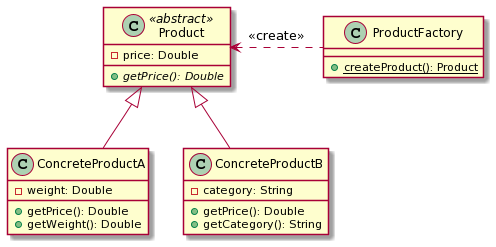
\includegraphics[scale=.7]{images/cld_factory_pattern.png}
\end{center}
	\caption{Veranschaulichung des Factory Method Patterns in einem Klassendiagramm}
\end{figure}

\subsection{Vorteile und Nachteile}
\paragraph{Vorteile}

\begin{itemize}
	\item Mit Hilfe des Factory Method Patterns können Unterklassen die Art, wie Objekte erstellt werden sollen, selbst wählen.
	\item Dieses Design Pattern fördert die lose Kopplung. Das heißt im Allgemeinen, dass anwendungsspezifische Klassen nicht mehr in den Code eingebunden werden müssen. 
	\item Die Kommunikation erfolgt ausschließlich über die Schnittstelle oder die abstrakte Klasse, so dass der Code mit allen Klassen funktioniert, die entweder die Schnittstelle implementieren oder die abstrakte Klasse erweitern.
\end{itemize}

\paragraph{Nachteile}

\begin{itemize}
	\item Falls die verwendeten Klassen nicht abstrakt sind, muss für jede individuelle Klasse eine Factory geschrieben werden.
\end{itemize}

\section{JavaScript Events und EventListener}
\paragraph{trix-initialize}\mbox{}\\
Sobald der \texttt{<trix-editor>} im DOM registriert wird und sein internes \texttt{Editor}-Objekt zur Benutzung bereit ist, wird das Event \texttt{trix-initialize} gefeuert.\\
Damit nicht die standardmäßig definierte Toolbar, sondern die erweiterte barrierefreie Toolbar, die diese ersetzen soll, angezeigt wird, ist es möglich auf dieses Event zu hören und dementsprechend darauf zu reagieren. Somit kann mit der Trix-Extension die Toolbar ersetzt werden, ohne dass der Endbenutzer etwas von diesem \\
DOM-Manipulationsprozess mitbekommt. % TODO: Formatierung

\paragraph{mousedown}\mbox{}\\
Das \texttt{mousedown} Event wird genau zu dem Zeitpunkt gefeuert, an dem sich der Mauszeiger auf einem HTML-Element befindet und dieses drückt.\\
Damit ein HTML-Button in der \texttt{<trix-toolbar>} aktiv ist und geklickt werden kann, hört dieser standardmäßig auf ein \texttt{mousedown} Event. Um diese Buttons mit einer Tastatur bedienen zu können, müsste der Trix-Editor im Quellcode auf Tastatureingaben reagieren und diese dementsprechend erneut validieren. In der Erweiterung Trix-Extension wird dieses Event künstlich ausgelöst mit \texttt{EventTarget.dispatchEvent()} und somit sind die Buttons in der Toolbar auch über die Tastatur bedienbar, ohne dass der Quellcode mit Wiederholung der Validation ergänzt werden muss.

\paragraph{keydown}\mbox{}\\
Wenn eine beliebige Taste gedrückt ist, wird das \texttt{keydown} Event gefeuert und liefert einen Code, der aussagt, welche Taste im Moment gedrückt wird.\\
Um den WYSIWYG Texteditor mittels einer Tastatur bedienen zu können, wird auf das \texttt{keydown} Event gelauscht. Je nachdem, welche Taste gedrückt wird, wird entweder der nächste oder der vorherige Button oder die Button-Gruppe fokussiert, geklickt oder der Fokus zur weiteren Texteingabe in den Editor gesetzt.\\

\newpage
\mbox{}\\
Folgende Tasten und Tastenkombinationen gelten in der Toolbar und im Editor:

\begin{table}[H]
	\begin{center}
	\begin{tabularx}{\textwidth}{| p{2.5cm} | l | X |}
		\hline
		\cellcolor{Gray}\textcolor{White}{Tasten} & \cellcolor{Gray}\textcolor{White}{Fokusbereich} & \cellcolor{Gray}\textcolor{White}{Beschreibung} \\
		\hline
		\texttt{ALT + F10} & \texttt{<trix-editor>} & Befindet sich der Fokus im Editor, dann gelangt man mit dieser Tastenkombination in die Toolbar
		und der erste vorkommende Button wird fokussiert.\\
		\hline
		\texttt{→ oder ↓} & \texttt{<trix-toolbar>} & Der nächste bzw. rechte Button in der Toolbar wird fokussiert.\\
		\hline
		\texttt{← oder ↑} & \texttt{<trix-toolbar>} & Der vorherige bzw. linke Button in der Toolbar wird fokussiert.\\
		\hline
		\texttt{STRG + →/↓} & \texttt{<trix-toolbar>} & Der erste Button der nächsten bzw. rechten Gruppe wird fokussiert.\\
		\hline
		\texttt{STRG + ←/↑} & \texttt{<trix-toolbar>} & Der erste Button der vorherigen bzw. linken Gruppe wird fokussiert.\\
		\hline
		\texttt{ENTER oder LEERTASTE} & \texttt{<trix-toolbar>} & Der aktuell fokussierte Button wird geklickt.\\
		\hline
		\texttt{ESC} & \texttt{<trix-toolbar>} & Befindet sich der Fokus in der Toolbar und wird die Taste gedrückt, so wird wieder der Editor fokussiert
		und der Cursor befindet sich an der zuletzt verwendeten Position.\\
		\hline
		\texttt{POS1} & \texttt{<trix-toolbar>} & Der erste in der Toolbar vorkommende Button wird fokussiert.\\
		\hline
		\texttt{ENDE} & \texttt{<trix-toolbar>} & Der letzte in der Toolbar vorkommende Button wird fokussiert.\\
		\hline
	\end{tabularx}
	\end{center}
	\caption{Tastenkombinationen zur Verwendung der Toolbar mit einer Tastatur}
\end{table}

\paragraph{focusout}\mbox{}\\
Sobald ein HTML-Element im Begriff dabei ist den Fokus zu verlieren, wird das \texttt{focusout} Event gefeuert.\\
Beim Initialisieren wird für jeden HTML-Button, der ein \texttt{DropdownButton}~\ref{dropdown_button} ist,  ein Dropdown Menü erstellt. Dieses Menü besteht aus einem HTML  \texttt{<div>} Element, in dem sich weitere HTML-Buttons befinden. Damit es für den Benutzer zu Beginn noch nicht sichtbar ist, erhält es das Attribut \texttt{hidden}. Sobald der \texttt{DropdownButton} geklickt wird, wird auch das Menü sichtbar und der Fokus auf den ersten Button darin gelegt. Wenn das Menü allerdings nicht mehr fokussiert ist, also das Event \texttt{focusout} gefeuert wird, erhält das Dropdown Menü erneut das Attribut \texttt{hidden} und wird somit für den Benutzer nicht mehr sichtbar sein.

\section{MutationObserver}
Der \texttt{MutationObserver} ist ein Interface, der Veränderungen in der Baumstruktur des DOMs beobachtet und wurde konzipiert, um die Mutation Events aus der DOM3 Events Spezifikation abzulösen.\\
Sobald die Toolbar geladen wird bzw. bestimmte Buttons geklickt werden, werden einige andere Buttons deaktiviert und erhalten das Attribut \texttt{disabled}. Dieses verhindert allerdings das Fokussieren eines Buttons, was mit dem Attribut \texttt{aria-disabled} problemlos funktioniert. Abhilfe verschafft deshalb ein \texttt{MutationObserver}. Erhält ein Button nun das Attribut \texttt{disabled}, beobachtet der \texttt{MutationObserver} diese Veränderung und entfernt es. Stattdessen fügt es das Attribut \texttt{aria-disabled} hinzu und setzt es auf \texttt{true}. Bei allen anderen Buttons, die nicht deaktiviert sind, ist \texttt{aria-disabled=false}.

\section{Delegation}
Die Delegation ist eine Alternative für die Vererbung. Vereinfacht wird die Aufgabe eines Objektes auf ein anderes Objekt verlagert (vgl. GeeksforGeeks 2018, \cite{delegation_2018}, 11.04.2021). Das kann so aufgefasst werden, dass die Methode des ursprünglichen Objektes die Methode des Zielobjektes aufruft. Ein Beispiel hierfür ist eine Basisklasse \texttt{Printer}, die die Klassen \texttt{RealPrinter} und \texttt{Computer} erbt. Somit ist diese Basisklasse in der Lage die Methode \texttt{print()} aufzurufen. Vererbung ist an und für sich eine gute Strategie, um Probleme zu lösen, sollte aber einen logischen Zusammenhang zwischen \texttt{parent} und \texttt{child} aufweisen können. Ein Beispiel für einen schlechten Zusammenhang ist, dass ein Auto einen Motor erbt. Stattdessen kann eine Assoziation solch eine Beziehung besser beschreiben als eine Vererbung (vgl. TU Wien 2013, \cite{tuv_delegation_2013}, 11.04.2021).

\begin{figure}[H]
\begin{center}
	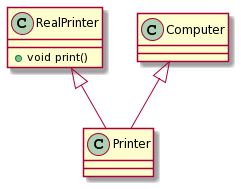
\includegraphics[scale=.7]{images/delegation-1.png}
\end{center}
	\caption{Ohne Delegation} 
\end{figure}

\begin{figure}[H]
\begin{center}
	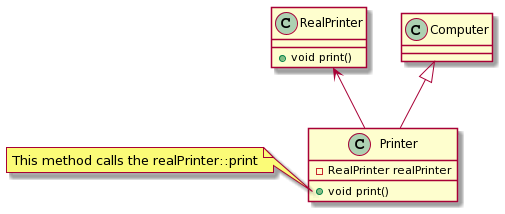
\includegraphics[scale=.7]{images/delegation-2.png}
\end{center}
	\caption{Mit Delegation} 
\end{figure}

\mbox{}\\
Im Rahmen der praktischen Arbeit dieser Diplomarbeit kann jedem \texttt{AttributeButton} kann die Identifikation eines HTML-Elements mitgegeben werden, das einen Dialog repräsentiert und bereits im HTML-Code erstellt worden ist. Die Delegation ermöglicht eine Kommunikation zwischen der Trix-Toolbar und dem Dialog. Sie dient ausschließlich dazu den Dialog zu öffnen und zu schließen, wobei zwei zusätzliche Funktionalitäten das Erstellen und das Entfernen von Links sind. Alles, was während oder nach dem Dialog geschieht, wird vom Entwickler selbst bestimmt.

\section{Barrierefreie Toolbar}

\subsection{Bedienbarkeit und Navigation}
Damit eine Toolbar für den Benutzer so barrierefrei wie möglich sein soll, gibt es einige bewährte Verfahrensweisen, 
die vom W3 Consortium empfohlen werden (vgl. W3C 2019, \cite{accessible_toolbar_2020}, 10.04.2021).

\paragraph{Tastaturanforderung}

\begin{itemize}
	\item Sobald in eine Toolbar tabuliert wird, soll das HTML-Element fokussiert werden, dass zuletzt im Fokus 
		gewesen ist. Wenn der Fokus auf anderes HTML-Element in der Toolbar gelegt wird, soll diese 
		Änderung mit dem HTML-Attribut \texttt{tabindex} gekennzeichnet sein. Das Element, das fokussiert wird 	
		oder ist, erhält den Wert 0 und alle anderen erhalten den Wert -1.
	\item Damit deaktivierte \texttt{<button>} Elemente zum Ausschneiden, Kopieren und Einfügen eines Textes in 
		den Texteditor von Screenreadern weiterhin erkannt werden, sollen sie fokussierbar bleiben. Damit weiß
		dem Benutzer, dass er diese Funktionen zu einem späteren Zeitpunkt nutzen kann.
	\item Innerhalb der Toolbar soll die Navigation mit den Pfeiltasten möglich sein. 
\end{itemize}

\paragraph{Gestaltung des Fokus}

\begin{itemize}
	\item Liegt der Fokus in der Toolbar, soll die Toolbar selbst anhand eines Rahmens hervorgehoben werden. Dies
		kennzeichnet dem Benutzer, dass eine Navigation mittels Pfeiltasten möglich ist.
	\item Wenn ein Element in der Toolbar selbst fokussiert ist, wird dieses nicht nur durch einen Rahmen 	
		hervorgehoben sondern auch durch eine andere Hintergrundfarbe.
\end{itemize}

\paragraph{Kennzeichnung von Buttons mit Pop-ups}

Gewisse Buttons, wie Textformatierungen, können über eine Kennzeichnung verfügen, die den Benutzern die
Funktionalitäten der Toolbar näher beschreibt. Dazu gehören Textformatierungen, wie fettgedruckt, kursiv, 
unterstrichen, rechtsbündig etc. 

\begin{itemize}
	\item Wenn ein Button eine Kennzeichnung besitzt, soll diese durch einen Fokus oder wenn sich der Mauszeiger
		über diesem Element befindet, wird die Beschreibung aufgedeckt.
	\item Die Beschreibung bleibt so lange sichtbar bis der Mauszeiger oder der Fokus nicht mehr auf dem Element 
		ist.
	\item Falls der Mauszeiger vom Element auf dessen Beschreibung wandert, bleibt diese aufgedeckt. 
\end{itemize}

\newpage
\paragraph{Unterstütze Funktionalitäten über die Tastatur}
~\begin{table}[H]
	\begin{center}
	\begin{tabular}{| c | m{10cm} |}
		\hline
 		\cellcolor{Gray}\textcolor{White}{Taste} & \cellcolor{Gray}\textcolor{White}{Funktionalität}  \\
		\hline
		\texttt{Tab} &
		\begin{itemize}
			\item Legt den Fokus auf und entfernt ihn aus der Toolbar
			\item Wenn die Toolbar nach dem Laden der Webseite zum ersten Mal fokussiert wird, erhält dessen 
				erstes Element den Fokus. Ansonsten wird der Fokus auf das zuletzt fokussierte Element gelegt.
		\end{itemize} \\
		\hline
		\texttt{rechte Pfeiltaste} &
		\begin{itemize}
			\item Bewegt den Fokus nach rechts auf das nächste Element.
			\item Ist das letzte Element am Ende der Toolbar fokussiert, erhält nun das erste Element den Fokus.
			\item Wenn ein Element in einem Pop-up Menü fokussiert ist, ist die Funktionalität dieser Taste 
				aufgehoben.
		\end{itemize} \\
		\hline
		\texttt{linke Pfeiltaste} &
		\begin{itemize}
			\item Bewegt den Fokus nach links auf das vorherige Element.
			\item Ist das erste Element am Anfang der Toolbar fokussiert, erhält nun das letzte Element den 
				Fokus.
			\item Wie bei der rechten Pfeiltaste, ist auch diese Funktionalität der Taste aufgehoben, sobald der
				Fokus in einem Pop-up Menü liegt.
		\end{itemize} \\
		\hline
		\texttt{Pos1} & Legt den Fokus auf das erste Element in der Toolbar \\
		\hline
		\texttt{Ende} & Legt den Fokus auf das letzte Element in der Toolbar \\
		\hline
		\texttt{Esc} & Falls die Beschreibung eines Buttons als Pop-up sichtbar ist, wird dieses wieder versteckt. \\
		\hline
	\end{tabular}
	\end{center}
	\caption{Unterstützte Funktionalitäten der Tastatur}
\end{table}

\paragraph{Schalten zwischen Buttons}\mbox{}\\
Damit eine Textformatierung auf den Text im Texteditor angewendet wird, kann mit der \texttt{Enter}-Taste oder mit 
der \texttt{Leertaste} zwischen den Buttons in der Toolbar gewechselt werden. Dieser ist dann entweder aktiv oder 
nicht aktiv.

\paragraph{Dropdown Menü}\mbox{}\\
Bei einem Dropdown Menü gibt es verschiedene Tasten, die verwendet werden können, um das Menü zu öffnen und einen Button darin auszuwählen.
 
 ~\begin{table}[H]
	\begin{center}
	\begin{tabular}{| m{4cm} | m{10cm} |}
		\hline
 		\cellcolor{Gray}\textcolor{White}{Taste} & \cellcolor{Gray}\textcolor{White}{Funktionalität}  \\
		\hline
		\texttt{Enter, Leertaste, Pfeil nach oben, Pfeil nach unten} & Öffnet das Dropdown Menü und legt den 
			Fokus auf einen Button in diesem Menü. Das ist entweder der aktuell aktive Button oder der erste 
			Button, der darin zu finden ist. \\
		\hline
		\texttt{Pfeil nach unten} &
		\begin{itemize}
			\item Fokusiert den nächsten Button im Menü
			\item Wenn es sich um den letzten Button im Menü handelt, wird der erste Button fokusiert.
		\end{itemize} \\
		\hline
		\texttt{Pfeil nach oben} &
		\begin{itemize}
			\item Fokusiert den vorherigen Button im Menü
			\item Wenn es sich um den ersten Button im Menü handelt, wird der letzte Button fokusiert.
		\end{itemize} \\
		\hline
		\texttt{Escape} & Schließt das Drowdown Menü und fokusiert den Button des Menüs in der Toolbar. \\
		\hline
	\end{tabular}
	\end{center}
	\caption{Unterstützte Funktionalitäten der Tastatur}
\end{table}

\paragraph{Links}\mbox{}\\
Empfohlen wird, dass sich ein Link mit \texttt{Enter} oder der  \texttt{Leertaste} öffnen lässt.  

\paragraph{ARIA Attribute}\mbox{}\\
Um eine Toolbar bestmöglich so zu gestalten, sodass diese für die meisten Menschen mit und ohne 
Einschränkungen zugänglich ist, können Accessible Rich Internet Applications (WAI-ARIA) Attribute zum Einsatz kommen (vgl. W3C 2006, \cite{wai_aria_2020}, 10.09.2020).  
Diese sind bei den meisten Screenreadern und Browsern implementiert und helfen insbesondere bei dynamischen 
Benutzeroberflächen. Beispiele hierfür sind Aktualisierung von Inhalten in Echtzeit, Hinweise oder Meldungen  bei 
Formularen oder auf der Webseite sowie die Navigation durch Webapplikationen. \\
Die wichtigsten ARIA Attribute für eine Toolbar sind in den folgenden Tabellen gelistet:

\newpage
\mbox{}\\
\textbf{Toolbar}
~\begin{longtable}{| p{.40\textwidth} | p{.60\textwidth} |} 
	\hline
	\cellcolor{Gray}\textcolor{White}{Rolle / ARIA Attribut} & \cellcolor{Gray}\textcolor{White}{Beschreibung}  \\
	\hline
	\begin{itemize}[label={}, leftmargin=*]
		\item \texttt{role='toolbar'}
		\item \texttt{<div>}
	\end{itemize} 
	& Dieses Attribut kennzeichnet das HTML-Element, das die Toolbar 
		repräsentieren soll als solche.  Der Container selbst ist nicht fokussierbar, sondern nur dessen Inhalt 
		über das Attribut \texttt{tabindex}\\
	\hline
	\begin{itemize}[label={}, leftmargin=*]
		\item \texttt{aria-label='Textformatierung'}
		\item \texttt{<div>}
	\end{itemize} 
	& Die Toolbar wird mit einem ansprechbaren Namen versehen. \\
	\hline
	\begin{itemize}[label={}, leftmargin=*]
		\item \texttt{aria-controls='IDREF'}
		\item \texttt{<div>}
	\end{itemize} 
	 & Dieses Attribut erhält den Wert, der auf das Textfeld verweist. Somit wird angegeben, dass dieses von der 
	 Toolbar kontrolliert wird. \\
	\hline
	\begin{itemize}[label={}, leftmargin=*]
		\item \texttt{tabindex='-1'}
		\item \texttt{<button>},
		\item \texttt{<div>},
		\item \texttt{<input type='checkbox'>},
		\item \texttt{<a>}
	\end{itemize} 
	& Es wird auf alle HTML-Elemente der Toolbar angewendet, außer auf die Element, die mit \texttt{TAB} navigiert 
	werden können. \\
	\hline
	\begin{itemize}[label={}, leftmargin=*]
		\item \texttt{tabindex='0'}
		\item \texttt{<button>},
		\item \texttt{<div>},
		\item \texttt{<input type='checkbox'>},
		\item \texttt{<a>}
	\end{itemize} 
	 & \begin{itemize}
		\item Mit dem Wert 0 wird indiziert, dass sich dieses HTML-Element mit der \texttt{TAB}-Taste navigieren 
		lässt.
		\item  Dieses Attribut mit diesem Wert wird nur auf ein HTML-Element in der Toolbar gesetzt.
		\item Sobald eine Webseite geladen wird, erhält standardmäßig das erste Element in der Toolbar dieses 
			Attribut.
		\item Wenn der Fokus auf ein andere Toolbar-Element gelegt wird, erhält dieses den Wert 0 und das 
			zuvor fokussierte Element den Wert -1.
	\end{itemize} \\
	\hline
	\begin{itemize}[label={}, leftmargin=*]
		\item \texttt{aria-pressed='true'} 
		\item \texttt{<button>}
	\end{itemize}
	& Gibt an, dass sich ein Button aktivieren und deaktivieren lässt sowie, dass die 	
		Textformatierung angewendet worden ist.\\
	\hline
	\begin{itemize}[label={}, leftmargin=*]
		\item \texttt{aria-pressed='false'}
		\item \texttt{<button>}
	\end{itemize}
	 & Gibt an, dass sich ein Button aktivieren und deaktivieren lässt sowie, dass die
		Textformatierung nicht angewendet worden ist.\\
	\hline
	\begin{itemize}[label={}, leftmargin=*]
		\item \texttt{aria-hidden='true'} 
		\item \texttt{<button>}
	\end{itemize}
	& Blendet das im zugänglichen Namen enthaltene Symbol aus\\
	\hline
	\begin{itemize}[label={}, leftmargin=*]
		\item \texttt{aria-disabled='true'} 
		\item \texttt{<button>}
	\end{itemize}
	& Ein HTML-Button erhält dieses Attribute mit dem Wert \texttt{true}, wenn dessen
		Funktionalität nicht verfügbar werden kann.\\
	\hline
	\begin{itemize}[label={}, leftmargin=*]
		\item \texttt{aria-disabled='false'} 
		\item \texttt{<button>}
	\end{itemize}
	& Ein HTML-Button erhält dieses Attribut mit dem Wert \texttt{false}, wenn dessen
		Funktonalität verfügbar ist. \\
	\hline
	\begin{itemize}[label={}, leftmargin=*]
		\item \texttt{} 
		\item \texttt{aria-label='Font: FONT FAMILY NAME'} 
		\item \texttt{<button>}
	\end{itemize}
	& Definiert einen zugänglichen Namen für den \texttt{<button>} im Menü und ändert seinen Wert auf den Wert
		zum \texttt{aria-label} des Buttons, der im Menü ausgewählt wird.\\
	\hline
	\begin{itemize}[label={}, leftmargin=*]
		\item \texttt{aria-haspopup='true'} 
		\item \texttt{<button>}
	\end{itemize}
	& Mit diesem Attribut wird angegeben, dass sich nach dem Klick auf den HTML-Button ein Pop-up-Menü 
	öffnet.\\
	\hline
	\begin{itemize}[label={}, leftmargin=*]
		\item \texttt{aria-controls='IDREF'} 
		\item \texttt{<button>}
	\end{itemize}
	& Der Wert dieses Attributes ist die Referenz auf das HTML-Element mit dem Attribut \texttt{role='menu'} und 
		gibt an, dass sich ein Menü öffnen oder schließen lässt.\\
	\hline
	\begin{itemize}[label={}, leftmargin=*]
		\item \texttt{aria-expanded='true'} 
		\item \texttt{<button>}
	\end{itemize}
	& \begin{itemize}[label={}, leftmargin=*]
		\item Wird erst dem \texttt{<button>} hinzugefügt, wenn das Menü offen ist und wieder entfernt, wenn sich
			das Menü wieder schließt.
		\item Gibt an, dass das Menü sichtbar ist und sich erst nach dem Aktivieren des Menü-Buttons wieder 
			schließt.
		\item Wird verwendet, damit Screenreader auf Touch-Geräten den Benutzern mitteilen kann, dass der
			HTML-Button berührt werden kann, wenn das Menü offen ist. Tastaturbenutzer können diesen
			Button hingegen nicht fokussieren, wenn das Menü offen ist.
	\end{itemize} \\
	\hline
	\begin{itemize}[label={}, leftmargin=*]
		\item \texttt{role='menu'} 
		\item \texttt{<ul>}
	\end{itemize}
	& Identifiziert das Menü, das weitere HTML-Buttons enthält.\\
	\hline
	\begin{itemize}[label={}, leftmargin=*]
		\item \texttt{aria-label='Font Family'} 
		\item \texttt{<ul>}
	\end{itemize}
	& Definiert den zugänglichen Namen des Menüs\\
	\hline
	\begin{itemize}[label={}, leftmargin=*]
		\item \texttt{role='menuitemradio'} 
		\item \texttt{<li>}
	\end{itemize}
	& Identifiziert das HTML-Listenelement, wobei der Textinhalt des HTML-Elementes zugleich der zugängliche
		Name ist.\\
	\hline
	\begin{itemize}[label={}, leftmargin=*]
		\item \texttt{aria-checked='true'} 
		\item \texttt{<li>}
	\end{itemize}
	& Besitzt ein \texttt{<button>} die Rolle \texttt{menuitemradio} wird mit diesem ARIA Attribut beim \texttt{<li>} 
		definiert, dass das ein HTML-Element ausgewählt ist und kann nur auf ein HTML-Element im jeweiligen 
		Menü angewendet werden.\\
	\hline
	\begin{itemize}[label={}, leftmargin=*]
		\item \texttt{aria-checked='true'} 
		\item \texttt{<li>}
	\end{itemize}
	& Besitzt ein \texttt{<button>} die Rolle \texttt{menuitemradio} wird mit diesem ARIA Attribut beim \texttt{<li>} 
		Element definiert, dass das ein HTML-Element nicht ausgewählt ist und wird auf alle HTML-Elemente im 
		jeweiligen Menü angewendet, die nicht ausgewählt sind.\\
	\hline
	\begin{itemize}[label={}, leftmargin=*]
		\item \texttt{tabindex='-1'} 
		\item \texttt{<li>}
	\end{itemize}
	& Besitzt ein \texttt{<button>} die Rolle \texttt{menuitemradio} wird mit diesem ARIA Attribut beim \texttt{<li>} 
		Element definiert, dass dieses fokussierbar ist. Im Normalfall erfolgt dies dynamisch mit JavaScript.\\
	\hline
	\caption{Wichtige Rollen und ARIA Attribute für die Webzugänglichkeit}
\end{longtable}

\subsection{Workarounds}

\paragraph{Unterstützung aller HTML-Tags}
\mbox{}\\
Eines der ersten Probleme, die im Rahmen dieser Diplomarbeit aufgetreten sind, ist die Tatsache, dass der 
\texttt{<trix-editor>} nur die HTML-Tags unterstützt, die in der Tabelle \ref{table:trix_supported_tags} festgelegt sind. 
Aus diesem Grund ist der Code für das Rendering geändert und dafür ein \texttt{TextAttribute}
~\ref{paragraph_textAttribute} erstellt worden, das ein Objekt zurückgibt. Im Normalfall würde der Texteditor dieses 
Objekt nicht erkennen, doch nach dem Ändern der Ansicht wird es das. Der überschriebene Code wird dann 
ausgeführt, wenn die Klasse \texttt{HTMLParser} aufgerufen wird. Dies geschieht beim Einfügen von HTML im 
Programm oder beim Initialisieren des Dokuments mit HTML. Die Funktion \texttt{sanitize()} aus der Klasse 
\texttt{HTMLSanitizer} musste ebenfalls überschrieben werden, da ansonsten nur fest kodierte HTML-Elemente 
zugelassen und das JavaScript-Protokoll verweigert werden.

\paragraph{Unterstützung von Tabellen und horizontalen Linien}
\mbox{}\\
Ein HTML \texttt{<table>} Element wird von Trix nicht unterstützt. Sobald eine Tabelle eingefügt wird, wird diese in 
Umbrüche und Pipes umgewandelt je nach Tabellenzeile und deren Inhalt. Um dieses Problem zu lösen, werden 
Tabellen in Trix Extension als einen Anhang betrachtet, da Trix mit Anhängen nichts anstellt und sie so belässt wie 
sie sind.\\
Bei einem \texttt{<hr>} Element gab es eine größere Herausforderung. Als erste Lösung wurde dieses HTML-
Element als \texttt{BlockAttribute}~\ref{paragraph_blockAttribute} registriert. Es stellte sich allerdings heraus, dass 
leere HTML-Elemente nicht unterstützt werden, weshalb \texttt{<hr>} zu geworden \texttt{<hr></hr>} ist. Deswegen 
wird auch hier das \texttt{<hr>} Element als Anhang betrachtet, wobei es in ein \texttt{<div>}-Tag eingepackt in 
\texttt{<trix-editor>} eingefügt wird. Alle anderen Anhänge werden hingegen in ein \texttt{<p>}-Tag gepackt.

\paragraph{Textformatierung beim Parsen eines Textes beibehalten}
\mbox{}\\
Beim Parsen von Absätzen in den \texttt{<trix-editor>} werden die Inhalte in ein \texttt{<div>} Element gegeben. Es hat sich herausgestellt, dass Trix eine Funktion besitzt, mit dem der Abstand zum Seitenrand überprüft wird. Falls der Abstand groß genug ist, fügt Trix eine zusätzliche leere Zeile ein. Da ein \texttt{<p>}-Tag einen größeren Abstand zum Seitenrad hat, werden unerwünschte Zeilenumbrüche eingebettet. Diese Funktion ist mit einer leeren überschrieben worden, um genau das zu vermeiden.

\subsection{Toolbar Replacer und Toolbar Replacer Factory}
\label{subsec_toolbar_replacer_factory}

Mit der Klasse \texttt{ToolbarReplacer} werden die Buttons in \texttt{<trix-toolbar>} ersetzt. Hierfür muss zunächst eine Factory erstellt werden. Erst dann kann eine \texttt{<trix-toolbar>} mit den neuen gruppierten Buttons erstellt werden.

\begin{figure}[H]
\begin{center}
	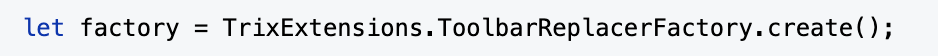
\includegraphics[scale=.7]{images/toolbar_replacer_factory.png}
\end{center}
	\caption{Erstellen einer Factory} 
\end{figure}

Nachdem die Buttons fertig definiert worden sind kann mit einem Objekt der Klasse \texttt{ToolbarReplacerFactory} 
die Methode \texttt{build()} aufgerufen werden, die ein Objekt der Klasse \texttt{ToolbarReplacer} zurückgibt. Es wird  
für jeden Button einen HTML-Button erstellt. Mit der Methode \texttt{attachToTrix()} können diese HTML-Buttons in  
\texttt{<trix-toolbar>} eingefügt werden, die mit ihrem \texttt{id}-Attribut oder als HTML-Element als Parameter 
übergeben wird.

\section{Button Elemente}
\label{subsec:buttons}
In dieser Erweiterung des Trix Texteditors wird zwischen vier verschiedenen Arten von Buttons unterschieden, wobei 
die  letzten beiden Buttons zusätzliche HTML-Buttons in der \texttt{<trix-toolbar>} darstellen und keine 
Funktionalitäten 
von Trix haben. Diese können mit \texttt{new TrixExtensions.<button class>(\{...\})} erstellt werden.

\begin{itemize}
	\item{\textbf{Action Button}} - \texttt{new TrixExtensions.ActionButton(\{...\})}
	\item{\textbf{Attribute Button}} - \texttt{new TrixExtensions.AttributeButton(\{...\})}
	\item{\textbf{Clickable Button}} - \texttt{new TrixExtensions.ClickableButton(\{...\})}
	\item{\textbf{Dropdown Button}} - - \texttt{new TrixExtensions.DropdownButton(\{...\})}
\end{itemize}

\mbox{}\\
Da es einige Attribute gibt, die in jedem HTML-Button von Trix zusätzlich zu dem Attribut \texttt{data-trix-attribute} 
oder 
\texttt{data-trix-action} enthalten sind, wurde im Rahmen dieser Diplomarbeit eine abstrakte Basisklasse 
\texttt{BaseButton} 
erstellt. Beim Erstellen eines HTML-Buttons können die folgenden Parameter definiert werden:

\begin{figure}[H]
\begin{center}
	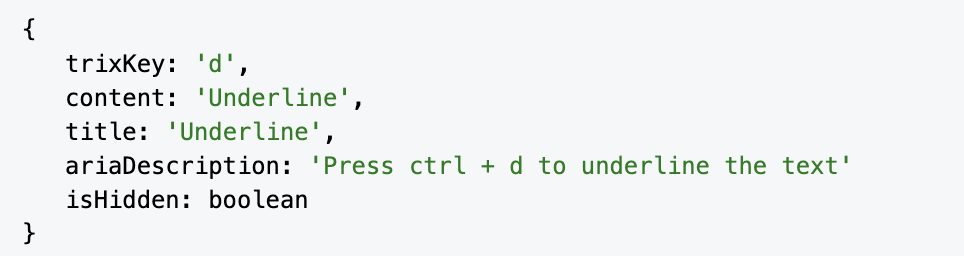
\includegraphics[scale=.7]{images/base-button.png}
\end{center}
	\caption{Standardparameter eines \texttt{<button>} Elementes}
\end{figure}

\begin{itemize}
	\item Mit \texttt{trixKey} wird ein Tastenkürzel festgelegt 
	\item \texttt{content} ist das \texttt{innerHTML} des Buttons
	\item \texttt{title} spezifiziert das gleichnamige HTML-Attribut des Buttons
	\item Die Beschreibung, die in \texttt{ariaDescription} angegeben wird, kann von einem Screenreader gelesen 
		werden und 
		trägt zur Barrierefreiheit des Texteditors bei.
	\item \texttt{isHidden} ist implementiert worden, da ein Dropdown Menü aus mehreren Buttons besteht und 
		diese für den Benutzer nicht sichtbar sein sollen, sofern der dazugehörige HTML-Button zum Einblenden 
		des Menüs nicht geklickt worden ist. Standardmäßig hat \texttt{isHidden} den Wert \texttt{false} und somit 
		ist der HTML-Button in der \texttt{<trix-toolbar>} sichtbar. Soll dieser nicht mehr sichtbar sein, wird der 
		Wert auf 
		\texttt{true} gesetzt.
\end{itemize}

\mbox{}\\
Der Texteditor Trix hat bereits einige \texttt{data-trix-attribute} und \texttt{data-trix-action} vordefiniert. Mit Hilfe von 
Trix Extension kann über die Klasse \texttt{StandardButtonManager} folgenderweise auf diese zugegriffen und optional 
der Wert verändert werden:

\begin{figure}[H]
\begin{center}
	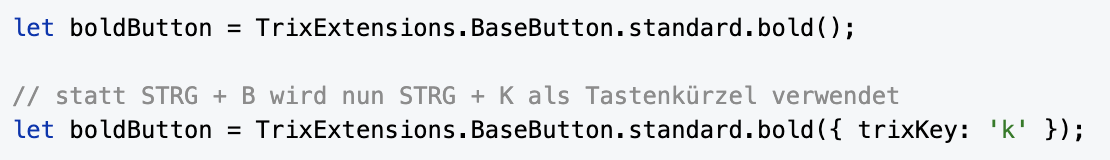
\includegraphics[scale=.7]{images/standard-button.png}
\end{center}
	\caption{Beispiel zum Erstellen eines Standard-Attribut-Buttons von Trix für einen fettgedruckten Text}
\end{figure}

\mbox{}\\
In der folgenden Tabelle sind alle vordefinierten Trix Attribute und Actions sowie alle HTML-Elemente, in denen der Text gewrappt wird oder Aktionen, die auf diesen ausgeführt werden, gelistet:

\begin{table}[H]
	\begin{center}
	\begin{tabularx}{\textwidth}{| p{4cm} | l | X |}
		\hline
		\cellcolor{Gray}\textcolor{White}{Trix Attribut/Action} & \cellcolor{Gray}\textcolor{White}{HTML-Element} & \cellcolor{Gray}\textcolor{White}{Beschreibung} \\
		\hline
		\hline
		\texttt{bold} & \texttt{<strong>} & fettgedruckter Text\\
		\hline
		\texttt{italic} & \texttt{<em>} & kursiver Text\\
		\hline
		\texttt{strike} & \texttt{<del>} & durchgestrichener Text\\
		\hline
		\texttt{href} & \texttt{<a>} & \texttt{<button>}, der ein Dialog für die Eingabe eines Links öffnet\\
		\hline
		\texttt{heading1} & \texttt{<h1>} & Überschrift der Ebene 1\\
		\hline
		\texttt{quote} & \texttt{<blockquote>} & Hervorheben eines Zitates\\
		\hline
		\texttt{code} & \texttt{<pre>} & Hervorheben eines Codeblocks\\
		\hline
		\texttt{bullet} & \texttt{<ul>} & Liste mit Aufzählungspunkten\\
		\hline
		\texttt{number} & \texttt{<ol>} & nummerierte Liste\\
		\hline
		\texttt{decreaseNestingLevel} & & Einrückung nach links\\
		\hline
		\texttt{increaseNestingLevel} & & Einrückung nach rechts\\
		\hline
		\texttt{attachFiles} & & Einfügen von Dateien, z. B. Bilder, Dokumente etc.\\
		\hline
		\texttt{undo} & & Formatierung oder Text rückgängig machen\\
		\hline
		\texttt{redo} & & Formatierung oder Text wiederherstellen\\
		\hline
	\end{tabularx}
	\end{center}
	\caption{In Trix vordefinierte Buttons}
	\label{table:trix_supported_tags}
\end{table}

\subsection{Action Button}
\label{subsec_action_button}

Bei einem Klick auf einen \texttt{<button>} mit dem Attribut \texttt{data-trix-action} wird eine bestimmte Aktion ausgeführt, die
bereits von Trix definiert worden ist. Aus diesem Grund kann keine weitere Aktion von dem Benutzer für einen Action Button erstellt 
werden. Beim Klick auf diesen HTML-Button mit einer selbstdefinierten \texttt{trixAction} würde die Aktion nicht funktionieren. \\
Stattdessen kann mit Trix Extension ein Clickable Button~\ref{subsec_clickable_button} erstellt werden, der übergebene 
Funktionen ausführt. 

\paragraph{Parameter eines Action Buttons}\mbox{}\\
\begin{figure}[H]
\begin{center}
	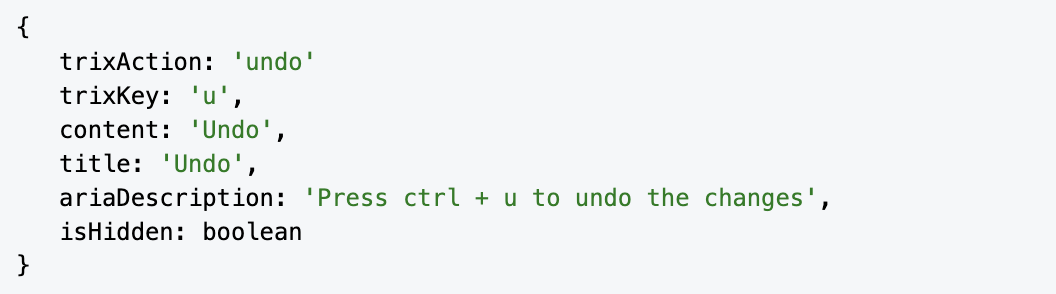
\includegraphics[scale=.7]{images/action-button.png}
\end{center}
	\caption{Beispiel eines Action Buttons, der die Formatierung oder den Text rückgängig macht}
\end{figure}

\mbox{}\\
Zusätzlich zu den Parametern, die in \texttt{BaseButton} definiert sind, gibt es \texttt{trixAction}. Hier ist der Wert einer der von Trix
vordefinierten Aktionen. Der Action Button findet ausschließlich im \texttt{StandardButtonManager} Verwendung und es können
keine selbstdefinierte Werte für \texttt{trixAction} festgelegt werden, da diese für den Texteditor unbekannt sind.

\newpage
\subsection{Attribute Button}
Bei Trix gibt es zwei Typen zum Formatieren des Textes: \texttt{textAttributes} und \\
\texttt{blockAttributes}. Wenn die gesamte Zeile gestaltet werden soll, werden \\
\texttt{blockAttributes} verwendet. Dazu zählen beispielsweise Überschriften (\texttt{<h1>} bis \texttt{<h6>}), Listen (\texttt{<ol>} 
und \texttt{<ul>}) etc.\\ Wenn stattdessen nur ein bestimmter Bereich des Textes formatiert werden soll, werden 
\texttt{textAttributes} verwendet. Das betrifft zum Beispiel kurisven Text, Schriftgrößen etc.\\
Diese Parameter beschreiben die standardmäßige Arbeitsweise der Button Elemente des Texteditors, die vor dem 
\texttt{<trix-editor>} erstellt werden.

\paragraph{Text Attribute}
\label{paragraph_textAttribute}\mbox{}\\
In der folgenden Abbildungen sind alle Eigenschaften für Textattribute ersichtlich:

\begin{figure}[H]
\begin{center}
	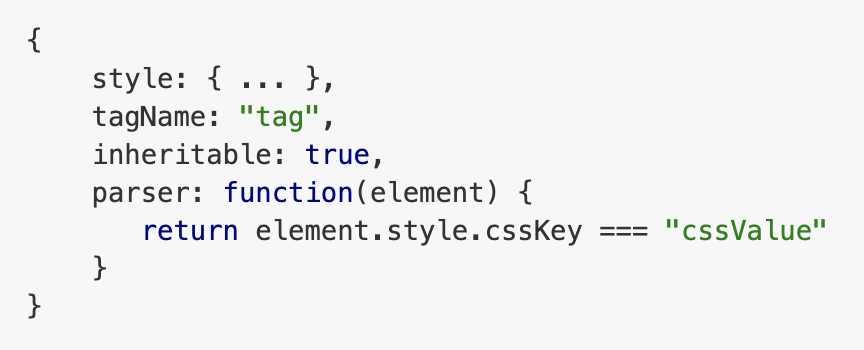
\includegraphics[scale=.7]{images/text_attributes.png}
\end{center}
	\caption{Eigenschaften eines \texttt{textAttributes}}
\end{figure}

\begin{itemize}
	\item In \texttt{style} kann ein beliebiger JavaScript Code zum Formatieren des Textes übergeben werden.
	\item Mit \texttt{tagName} wird festgelegt, in welches HTML-Tag der gestaltete Text gewrappt wird.
	\item \texttt{inheritable} spezifiziert, ob die Formatierung so lange verwendet werden soll bis der Attribute Button wieder deaktiviert wird (Wert: \texttt{true}) oder nur für ein Zeichen gilt (Wert: \texttt{false}). 
	\item Der \texttt{parser} muss nur gesetzt werden, wenn die Eigenschaft \texttt{style} ebenfalls festgelegt wurde. Dadurch behält ein Text, der mit dieser Formatierung kopiert und eingefügt wird, diese bei.
\end{itemize}

\begin{figure}[H]
\begin{center}
	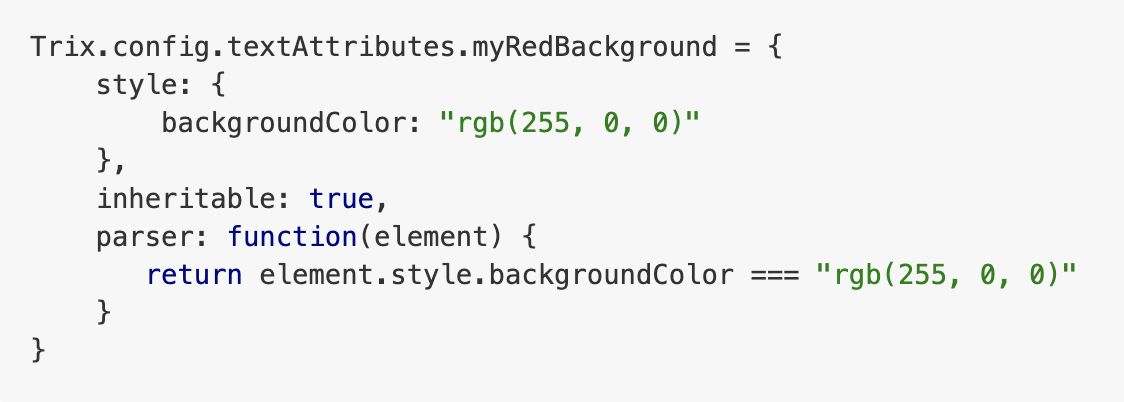
\includegraphics[scale=.7]{images/text_attributes_example.png}
\end{center}
	\caption{Beispiel eines \texttt{textAttributes}, der den Text im \texttt{<trix-editor>} einen roten Hintergrund gibt}
\end{figure}

\paragraph{Block Attribute}
\label{paragraph_blockAttribute}\mbox{}\\
Beim Texteditor Trix wird der Text immer in Blöcke gewrappt. Wenn ein dreizeiliger Text verfasst wurde, bedeutet das somit, dass diese drei Zeilen einen gemeinsamen Block bilden, der nach Belieben formatiert werden kann. Um ein Blockattribut anzuwenden, muss nicht unbedingt die gesamte Zeile markiert werden. Die Formatierung wird automatisch auf die Zeile angewendet, in dem sich der Cursor befindet.\\
Angenommen aus der ersten Zeile soll eine Überschrift werden. Durch das Styling wird der Block mit den drei Zeilen nun in einen Block mit dem HTML-Heading-Tag und einen Block mit den anderen restlichen zwei Zeilen getrennt.\\
Folgende Parameter können für Blockattribute festgelegt werden:

\begin{figure}[H]
\begin{center}
	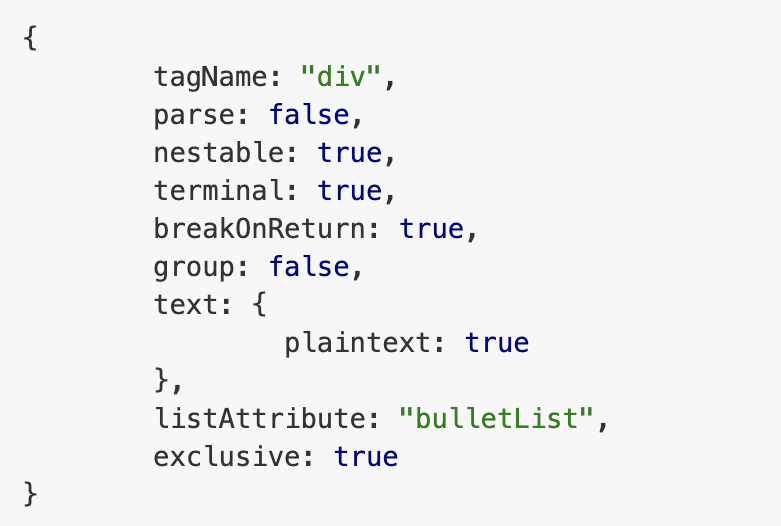
\includegraphics[scale=.7]{images/block_attributes.png}
\end{center}
	\caption{Eigenschaften eines \texttt{blockAttributes}}
\end{figure}

\begin{itemize}
	\item Wie bei \texttt{textAttributes} kann bei der Eigenschaft \texttt{tagName} ein gültiges HTML-Tag festgelegt werden, in dem der Block gewrappt werden soll. 
	\item Bei \texttt{parse} kann mit den Werten \texttt{true} oder \texttt{false} oder angegeben werden, ob ein kopierter Text dieselbe Formatierung des Blocks beibehält oder nicht.
	\item Mit \texttt{nestable} kann der Text mit dem Blockattribut in ein anderes HTML-Tag verschachtelt werden. 
	\item \texttt{terminal} gibt an, ob dieses Blockattribut mit anderen kombiniert werden kann. Ist der Wert \texttt{true}, können keine anderen Blockattribute angewendet werden und andere Attribute Buttons mit \texttt{blockAttributes} sind deaktiviert.
	\item Soll die Formatierung nach einmal tätigen der Enter-Taste abgebrochen werden, muss \texttt{breakOnReturn} auf \texttt{true} gesetzt werden. Ansonsten müsste die Enter-Taste zweimal getätigt werden.
	\item Damit das HTML-Element in ein anderes HTML-Tag als Teil einer Liste gewrappt wird, kann bei \texttt{listAttribute} der Name eines anderen Blockattributes angegeben werden.
\end{itemize}

\begin{figure}[H]
\begin{center}
	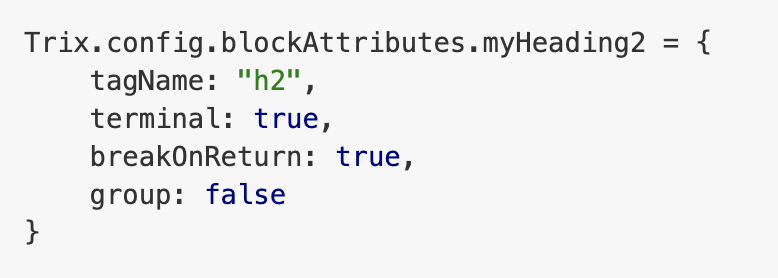
\includegraphics[scale=.7]{images/block_attributes_example.png}
\end{center}
	\caption{Beispiel eines \texttt{blockAttributes}, der den Text als Überschrift im HTML-Heading-Tag \texttt{<h2>} wrappt}
\end{figure}

\paragraph{Parameter eines Attribute Buttons}\mbox{}\\

\begin{figure}[H]
\begin{center}
	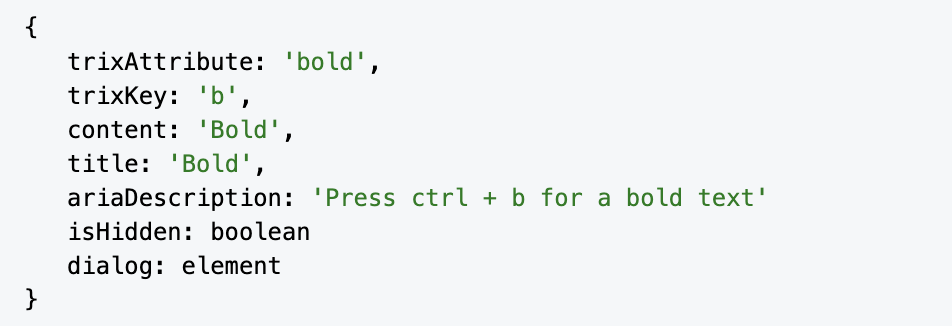
\includegraphics[scale=.7]{images/attribute-button.png}
\end{center}
	\caption{Eigenschaften eines Attribute Buttons}
\end{figure}

\mbox{}\\
Hier gibt es zusätzlich zu den Parametern, die in \texttt{BaseButton} definiert sind, die Eigenschaften \texttt{trixAttribute} und 
\texttt{dialog}. \\
\texttt{trixAttribute} kann entweder ein von Trix bereitgestelltes oder ein selbstdefiniertes \texttt{textAttribute} oder 
\texttt{blockAttribute} sein. \\
Soll der Benutzer nach dem Klick auf einen \texttt{<button>} mit einem Pop-up-Dialog interagieren, kann optional zusätzlich in
\texttt{dialog} noch ein Dialog in Form eines HTML-Elementes mit einer eindeutigen Identifikation mitgegeben werden.

\begin{figure}[H]
\begin{center}
	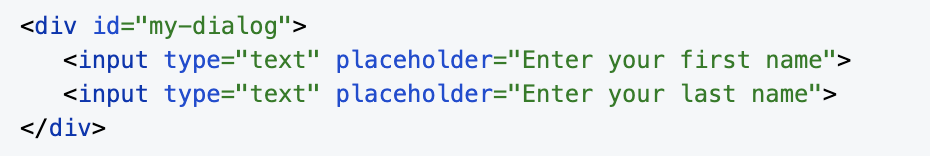
\includegraphics[scale=.7]{images/dialog-example.png}
\end{center}
	\caption{Beispiel eines Dialogs}
\end{figure}

\begin{figure}[H]
\begin{center}
	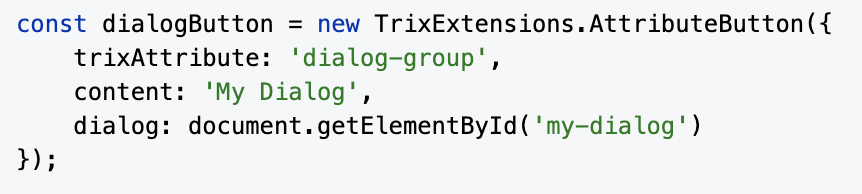
\includegraphics[scale=.7]{images/attribute-button-dialog-example.png}
\end{center}
	\caption{Beispiel eines Attribute Buttons mit einem Dialog mit Eingabefeldern}
\end{figure}

\mbox{}\\
Wenn ein Dialog mitgegeben wird, wird das spezifizierte HTML-Element durch Trix Extension in ein \texttt{<div>} gewrappt, 
welches dann Zugriff auf die \texttt{delegate} Klasse \texttt{DialogDelegate} hat. \\
Folgende Funktionen können bei einem Dialog ausgeführt werden:

\begin{itemize}
	\item \texttt{close(dialog)} schließt das zur Verfügung gestellte Dialog.
	\item \texttt{link(href)} erstellt einen Link mit dem selektierten Text als String-Parameter. Falls nichts selektiert wird, wird an
		der Stelle des Cursors der Link als Text eingefügt.
	\item \texttt{unlink()} entfernt den Link vom selektierten Text, falls möglich.
\end{itemize}

\subsection{Clickable Button}
\label{subsec_clickable_button}

Wie im Abschnitt \ref{subsec_action_button} bereits erwähnt worden ist, können keine weiteren Action Buttons erstellt werden, da der Texteditor Trix diese nicht erkennen kann. Abhilfe hierfür, um dennoch benutzerdefinierte Funktionen, wie Kopieren, Ausschneiden etc., ausführen zu können, bietet der Clickable Button von Trix Extension.

\begin{figure}[H]
\begin{center}
	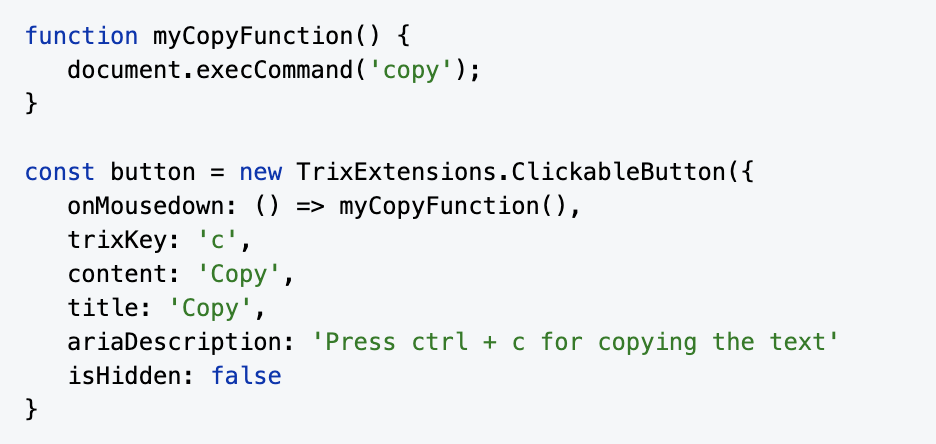
\includegraphics[scale=.7]{images/clickable-button-example.png}
\end{center}
	\caption{Beispiel eines Clickable Buttons, der den selektierten Text kopiert}
\end{figure}

\mbox{}\\
Neben den \texttt{BaseButton}-Eigenschaften muss beim Parameter \texttt{onMousedown} eine Funktion mitgegeben 
werden.
Der zu der \texttt{<trix-toolbar>} hinzugefügte HTML-Button hört nun auf das JavaScript Event \texttt{mousedown}.
Sobald der \texttt{<button>} geklickt worden ist, wird das JavaScript Event ausgelöst und die im Parameter 
übergebene Funktion ausgeführt.

\subsection{Dropdown Button}
\label{dropdown_button}

Mit Hilfe des Dropdown Buttons wird ein \texttt{<button>} mit einem Dropdown Menü in der \texttt{<trix-toolbar>} 
erstellt.

\begin{figure}[H]
\begin{center}
	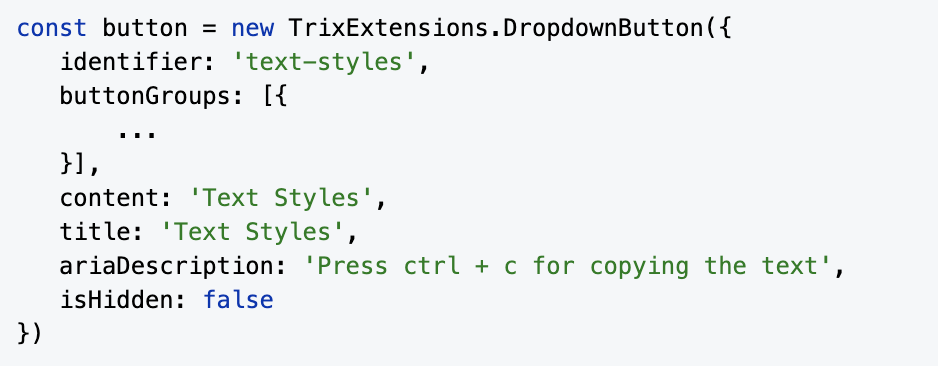
\includegraphics[scale=.7]{images/dropdown-button-example.png}
\end{center}
	\caption{Beispiel eines Dropdown Buttons}
\end{figure}

\mbox{}\\
Neben den Parametern aus \texttt{BaseButton} wird im Parameter \texttt{identifier} eine eindeutige Identifikation für
den in \texttt{<trix-toolbar>} hinzugefügten \texttt{<button>} festgelegt. \\
Im Parameter \texttt{buttonGroups}, der ein Array ist, werden Buttons definiert, die jeweils als \texttt{<button>} im 
Dropdown Menü in einem ungeordneten HTML-Listen-Element platziert werden. Wird der Dropdown Button geklickt, 
wird das Menü eingeblendet.

\subsection{Gruppierung der Buttons}

Die einzelnen \texttt{<button>} Elemente in der \texttt{<trix-toolbar>} müssen gruppiert werden, ansonsten gibt es 
einen Error. Hierfür muss zuvor eine Factory erstellt werden, wie im Abschnitt~\ref{subsec_toolbar_replacer_factory}. 
Mit dieser können die HTML-Buttons in einem \texttt{<span>} von anderen Gruppen getrennt werden. \\
Eine \texttt{ButtonGroup} die folgenden Parameter:

\begin{figure}[H]
\begin{center}
	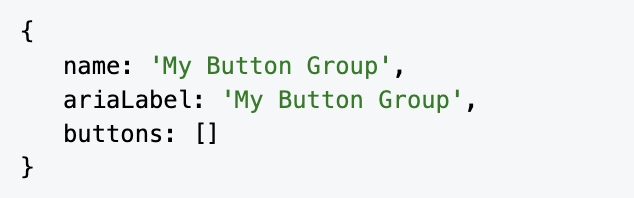
\includegraphics[scale=.7]{images/button-group.png}
\end{center}
	\caption{Parameter einer Button Group}
\end{figure}

\begin{itemize}
	\item \texttt{name} kennzeichnet die eindeutige Bezeichnung der Button Group.
	\item Optional kann ein \texttt{ariaLabel} mitgegeben werden. Der \texttt{<span>} erhält dann das Attribut
		\texttt{aria-label}, um zusätzliche Barrierefreiheit bereitzustellen.
	\item Im Array \texttt{buttons} können mehrere Buttons definiert werden, die gemeinsam eine Gruppe in der
		\texttt{<trix-toolbar>} bilden.
\end{itemize}

\mbox{}\\
Es gibt zwei Arten wie eine Button Group erstellt werden kann:

\begin{itemize}
	\item 1. Die Gruppe wird direkt mit der Factory erstellt und zur \texttt{<trix-toolbar>} hinzugefügt.
	\item 2. Die Gruppe wird separat als Objekt erstellt und erst später der Factory übergeben und zur 
		\texttt{<trix-toolbar>} hinzugefügt.
\end{itemize}

\begin{figure}[H]
\begin{center}
	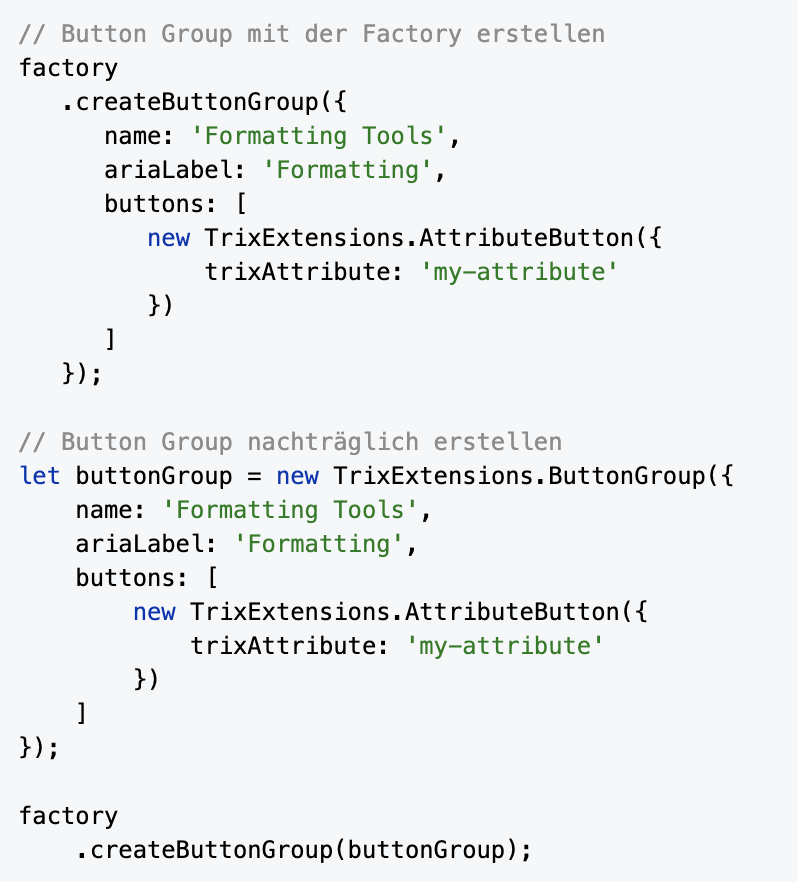
\includegraphics[scale=.7]{images/button-group-example.png}
\end{center}
	\caption{Beispiel zum Erstellen einer Button Group}
\end{figure}